\documentclass{article} 
\usepackage{tikz}
\usetikzlibrary{decorations.pathmorphing,patterns}
\begin{document}
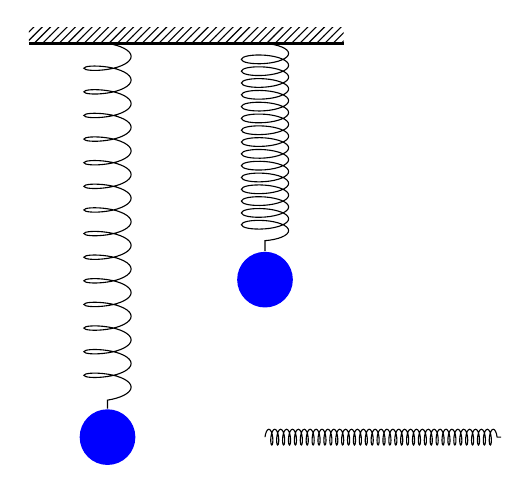
\begin{tikzpicture}
\node[circle,fill=blue,inner sep=2.5mm] (a) at (0,0) {};
\node[circle,fill=blue,inner sep=2.5mm] (b) at (2,2) {};
\draw[decoration={aspect=0.3, segment length=3mm, amplitude=3mm,coil},decorate] (0,5) -- (a); 
\draw[decoration={aspect=0.3, segment length=1.5mm, amplitude=3mm,coil},decorate] (2,5) -- (b); 
\draw[decoration={aspect=0.3, segment length=.75mm, amplitude=1mm,coil},decorate] (2,0) -- (5,0); 
\fill [pattern = north east lines] (-1,5) rectangle (3,5.2);
\draw[thick] (-1,5) -- (3,5);
\end{tikzpicture}
\end{document}